\documentclass[12pt,letterpaper]{article}
\usepackage{graphicx,textcomp}
\usepackage{natbib}
\usepackage{setspace}
\usepackage{fullpage}
\usepackage{color}
\usepackage[reqno]{amsmath}
\usepackage{amsthm}
\usepackage{fancyvrb}
\usepackage{amssymb,enumerate}
\usepackage[all]{xy}
\usepackage{endnotes}
\usepackage{lscape}
\newtheorem{com}{Comment}
\usepackage{float}
\usepackage{hyperref}
\newtheorem{lem} {Lemma}
\newtheorem{prop}{Proposition}
\newtheorem{thm}{Theorem}
\newtheorem{defn}{Definition}
\newtheorem{cor}{Corollary}
\newtheorem{obs}{Observation}
\usepackage[compact]{titlesec}
\usepackage{dcolumn}
\usepackage{tikz}
\usetikzlibrary{arrows}
\usepackage{multirow}
\usepackage{xcolor}
\newcolumntype{.}{D{.}{.}{-1}}
\newcolumntype{d}[1]{D{.}{.}{#1}}
\definecolor{light-gray}{gray}{0.65}
\usepackage{url}
\usepackage{listings}
\usepackage{color}

\definecolor{codegreen}{rgb}{0,0.6,0}
\definecolor{codegray}{rgb}{0.5,0.5,0.5}
\definecolor{codepurple}{rgb}{0.58,0,0.82}
\definecolor{backcolour}{rgb}{0.95,0.95,0.92}

\lstdefinestyle{mystyle}{
	backgroundcolor=\color{backcolour},   
	commentstyle=\color{codegreen},
	keywordstyle=\color{magenta},
	numberstyle=\tiny\color{codegray},
	stringstyle=\color{codepurple},
	basicstyle=\footnotesize,
	breakatwhitespace=false,         
	breaklines=true,                 
	captionpos=b,                    
	keepspaces=true,                 
	numbers=left,                    
	numbersep=5pt,                  
	showspaces=false,                
	showstringspaces=false,
	showtabs=false,                  
	tabsize=2
}
\lstset{style=mystyle}
\newcommand{\Sref}[1]{Section~\ref{#1}}
\newtheorem{hyp}{Hypothesis}

\title{Problem Set 3}
\date{Due: November 19, 2022}
\author{Applied Stats/Quant Methods 1}


\begin{document}
	\maketitle
	\section*{Instructions}
	\begin{itemize}
		\item Please show your work! You may lose points by simply writing in the answer. If the problem requires you to execute commands in \texttt{R}, please include the code you used to get your answers. Please also include the \texttt{.R} file that contains your code. If you are not sure if work needs to be shown for a particular problem, please ask.
	\item Your homework should be submitted electronically on GitHub.
	\item This problem set is due before 23:59 on Sunday November 19, 2023. No late assignments will be accepted.

	\end{itemize}

		\vspace{.25cm}
	
\noindent In this problem set, you will run several regressions and create an add variable plot (see the lecture slides) in \texttt{R} using the \texttt{incumbents\_subset.csv} dataset. Include all of your code.
\begin{verbatim}
	First i want to apologise because my scatterplots are all over the place. 
	I am aware I might lose points for it but I tried many ways to imput them 
	and they keept showing up in random places. I am sorry because it looks messy.
\end{verbatim}

	\vspace{.1cm}
\section*{Question 1}
\vspace{.25cm}
\noindent We are interested in knowing how the difference in campaign spending between incumbent and challenger affects the incumbent's vote share. 
	\begin{enumerate}
		\item Run a regression where the outcome variable is \texttt{voteshare} and the explanatory variable is \texttt{difflog}.
		\begin{verbatim}
			Code for the regression and the summary to be able to see the results.
		\end{verbatim}
		\begin{lstlisting}
			model <- lm(voteshare~difflog, data=inc.sub)
			summary(model)
	    \end{lstlisting}
		\begin{verbatim}
			Output:
			Residuals:    
			Min -0.26832   1Q -0.05345   Median -0.00377   3Q 0.04780   Max 0.32749 
			Coefficients:           
			            Estimate  Std. Error  t value  Pr(>|t|)    
			(Intercept) 0.579031   0.002251  257.19   <2e-16 ***
			difflog     0.041666   0.000968   43.04   <2e-16 ***
			Residual standard error: 0.07867 on 3191 degrees of freedom
			Multiple R-squared:  0.3673,	Adjusted R-squared:  0.3671 
			F-statistic:  1853 on 1 and 3191 DF,  p-value: < 2.2e-16
		\end{verbatim}
		\item Make a scatterplot of the two variables and add the regression line. 
		\begin{verbatim}
			Code for plotting the two variables and then adding the regression line.
		\end{verbatim}
		\begin{lstlisting}
			plot(x=inc.sub$difflog, y=inc.sub$voteshare)
			abline(model)
		\end{lstlisting}
		\begin{figure}
			\vspace{-1cm}
			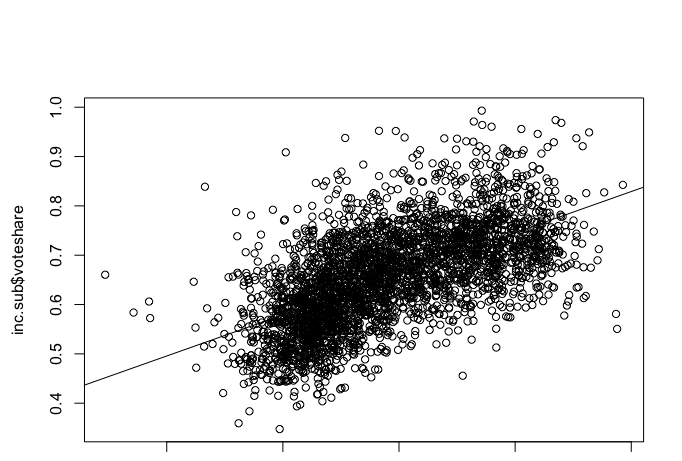
\includegraphics[width=15cm]{Rplotex1.png}
			\caption{Voteshare X Difflog}
		\end{figure}	
		\item Save the residuals of the model in a separate object.
		\begin{verbatim}
			I saved the residuals from the first model as residuals_1
			I also printed just to make sure I had saved them.
		\end{verbatim}
		 \begin{lstlisting}
			residuals_1 <- residuals(model)
			print(residuals_1)
		\end{lstlisting}
		\item Write the prediction equation.
		\begin{verbatim}
			Regression equation for x being the variable difflog, b0 the intercept 
			and b1 the slope as seen in the output from the model's summary.
		\end{verbatim}
		\begin{equation}
			\hat{y} = b_0 + b_1x
		\end{equation}
		\begin{equation}
			\hat{y} = 0.58 + 0.04*difflog
		\end{equation}
	\end{enumerate}
	
\newpage

\section*{Question 2}
\noindent We are interested in knowing how the difference between incumbent and challenger's spending and the vote share of the presidential candidate of the incumbent's party are related.	\vspace{.25cm}
	\begin{enumerate}
		\item Run a regression where the outcome variable is \texttt{presvote} and the explanatory variable is \texttt{difflog}.
		\begin{verbatim}
			Code for the regression and the summary to be able to see the results.
		\end{verbatim}
		\begin{lstlisting}
			model_2 <- lm(presvote~difflog, data=inc.sub)
			summary(model_2)
		\end{lstlisting}
		\begin{verbatim}
			Residuals:     
			Min -0.32196  1Q-0.07407  Median-0.00102   3Q 0.07151   Max 0.42743 
			Coefficients:          
			            Estimate   Std. Error t value  Pr(>|t|)    
			(Intercept) 0.507583   0.003161  160.60   <2e-16 ***
			difflog     0.023837   0.001359   17.54   <2e-16  
			Residual standard error: 0.1104 on 3191 degrees of freedom
			Multiple R-squared:  0.08795,	
			Adjusted R-squared:  0.08767 
			F-statistic: 307.7 on 1 and 3191 DF,  p-value: < 2.2e-16
		\end{verbatim}
		\item Make a scatterplot of the two variables and add the regression line. 
		\begin{verbatim}
			Code for plotting the two variables and then adding the regression line.
		\end{verbatim}
		\begin{lstlisting}
			plot(x=inc.sub$difflog, y= inc.sub$presvote)
			abline(model_2)
		\end{lstlisting}
		\begin{figure}
			\vspace{-1cm}
			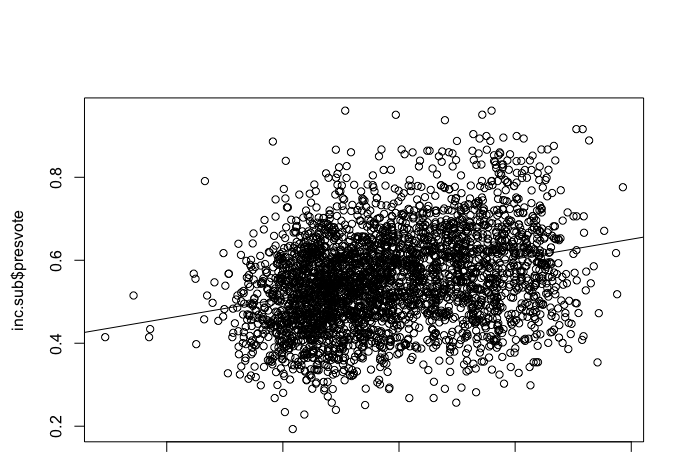
\includegraphics[width=15cm]{Rplot2im.png}
			\caption{Presvote X Difflog}
		\end{figure}
		\item Save the residuals of the model in a separate object.
		\begin{verbatim}
			I saved the residuals of model_2 as residuals_2
			I also printed just to make sure I had saved them.
		\end{verbatim}
		\begin{lstlisting}
		residuals_2 <- residuals(model_2)
		print(residuals_2)
		\end{lstlisting}	
		\item Write the prediction equation.
		\begin{verbatim}
			Regression equation for x being the variable difflog, b0 the intercept 
			and b1 the slope as seen in the output from the model_2's summary.
		\end{verbatim}
		\begin{equation}
			\hat{y} = b_0 + b_1x
		\end{equation}
		\begin{equation}
			\hat{y} = 0.50 + 0.02*difflog
		\end{equation}
	\end{enumerate}
			
	\newpage	
\section*{Question 3}

\noindent We are interested in knowing how the vote share of the presidential candidate of the incumbent's party is associated with the incumbent's electoral success.
	\vspace{.25cm}
	\begin{enumerate}
		\item Run a regression where the outcome variable is \texttt{voteshare} and the explanatory variable is \texttt{presvote}.
		\begin{verbatim}
			Code for the regression and the summary to be able to see the results.
		\end{verbatim}
		\begin{lstlisting}
			model_3 <- lm(voteshare~presvote, data=inc.sub)
			summary(model_3)
		\end{lstlisting}
	   \begin{verbatim} 
			Residuals:    
			Min -0.27330  1Q -0.05888  Median 0.00394 3Q 0.06148  Max 0.41365 
			Coefficients:            
		        	   Estimate   Std. Error  t value   Pr(>|t|)    
			(Intercept) 0.441330   0.007599   58.08   <2e-16 ***
			presvote    0.388018   0.013493   28.76   <2e-16 ***
			
			Residual standard error: 0.08815 on 3191 degrees of freedom
			Multiple R-squared:  0.2058,	Adjusted R-squared:  0.2056
			F-statistic:   827 on 1 and 3191 DF,  p-value: < 2.2e-16
		\end{verbatim}
		\item Make a scatterplot of the two variables and add the regression line. 
		\begin{verbatim}
			Code for plotting the two variables and then adding the regression line.
		\end{verbatim}
		\begin{lstlisting}
			plot(x=inc.sub$presvote, y=inc.sub$voteshare)
			abline(model_3)
		\end{lstlisting}
		 \begin{figure}
			\vspace{-1cm}
			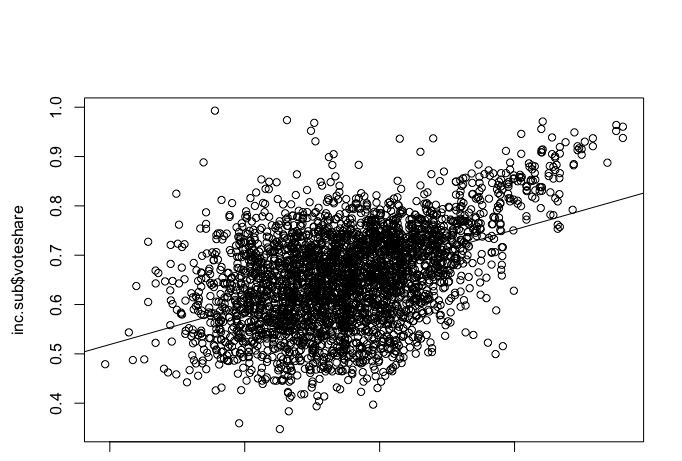
\includegraphics[width=15cm]{Rplot3.png}
			\caption{ voteshare X presvote}
		\end{figure}
		\item Write the prediction equation.
		\begin{verbatim}
			Regression equation for x being the variable presvote, b0 the intercept 
			and b1 the slope as seen in the output from the model_3's summary.
		\end{verbatim}
		\begin{equation}
			\hat{y} = b_0 + b_1x
		\end{equation}
		\begin{equation}
			\hat{y} = 0.44 + 0.38*presvote
		\end{equation}
	\end{enumerate}

\newpage	
\section*{Question 4}
\noindent The residuals from part (a) tell us how much of the variation in \texttt{voteshare} is $not$ explained by the difference in spending between incumbent and challenger. The residuals in part (b) tell us how much of the variation in \texttt{presvote} is $not$ explained by the difference in spending between incumbent and challenger in the district.
	\begin{enumerate}
		\item Run a regression where the outcome variable is the residuals from Question 1 and the explanatory variable is the residuals from Question 2.	
		\begin{verbatim}
			Code for the regression using the saved objects with residuals from 
			the first model and model_2 and the summary to be able to see the results.
		\end{verbatim}
		\begin{lstlisting}
		model_4 <- lm(residuals_1~residuals_2)
		summary(model_4)
		\end{lstlisting}
		\begin{verbatim}
	Residuals:    
	Min -0.25928 1Q -0.04737  Median -0.00121  3Q  0.04618     Max  0.33126 
	Coefficients:             
	             Estimate   Std. Error  t value  Pr(>|t|)    
	(Intercept) -1.942e-18  1.299e-03    0.00        1    
	residuals_2  2.569e-01  1.176e-02   21.84   <2e-16 ***
	---Signif. codes:  0 ‘***’ 0.001 ‘**’ 0.01 ‘*’ 0.05 ‘.’ 0.1 ‘ ’ 1
	Residual standard error: 0.07338 on 3191 degrees of freedom
	Multiple R-squared:   0.13,	Adjusted R-squared:  0.1298 
	F-statistic:   477 on 1 and 3191 DF,  p-value: < 2.2e-16
		\end{verbatim}
		\item Make a scatterplot of the two residuals and add the regression line. 	
		\begin{verbatim}
			Code for plotting the two residuals and then adding the regression line.
		\end{verbatim}
		\begin{lstlisting}
			plot(x=residuals_2, y=residuals_1)
			abline(model_4)
			\end{lstlisting}
		\begin{figure}
			\vspace{-1cm}
			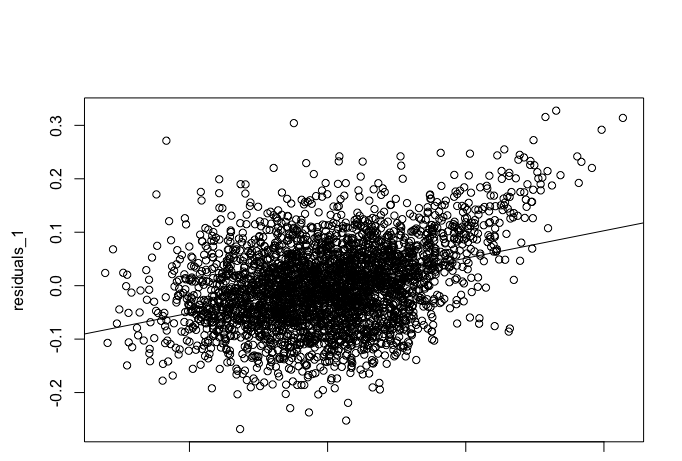
\includegraphics[width=15cm]{Rplot4b.png}
			\caption{ residuals model 1 X residuals model 2}
		\end{figure}	
		\item Write the prediction equation.
		\begin{verbatim}
			Regression equation for x being residuals_2, b0 the intercept 
			and b1 the slope as seen in the output from the model_4's summary.
		\end{verbatim}
			\begin{equation}
			\hat{y} = b_0 + b_1x
		\end{equation}
		\begin{equation}
			\hat{y} =  -1.94 + 2.56 *ressiduals_2
		\end{equation}
	\end{enumerate}
	
	\newpage	

\section*{Question 5}
\noindent What if the incumbent's vote share is affected by both the president's popularity and the difference in spending between incumbent and challenger? 
	\begin{enumerate}
		\item Run a regression where the outcome variable is the incumbent's \texttt{voteshare} and the explanatory variables are \texttt{difflog} and \texttt{presvote}.
		\begin{verbatim}
			Code for the regression and the summary to be able to see the results.
		\end{verbatim}
		\begin{lstlisting}
			model_5 <- lm(voteshare~difflog+presvote,data=inc.sub)
			summary(model_5)
		\end{lstlisting}
		\begin{verbatim}
			Residuals: 
			Min -0.25928  1Q -0.04737 Median -0.00121  3Q 0.04618  Max 0.33126 
			Coefficients:             
		            Estimate  Std. Error  t value Pr(>|t|)   
			(Intercept) 0.4486442  0.0063297   70.88   <2e-16 ***
			difflog     0.0355431  0.0009455   37.59   <2e-16 ***
			presvote    0.2568770  0.0117637   21.84   <2e-16 ***
			Residual standard error: 0.07339 on 3190 degrees of freedom
			Multiple R-squared:  0.4496,	Adjusted R-squared:  0.4493 
			F-statistic:  1303 on 2 and 3190 DF,  p-value: < 2.2e-16
		\end{verbatim}
		\item Write the prediction equation.
		\begin{verbatim}
		Regression equation for x1 being the variable difflog and x2 being the variable
		presvote, b0 the intercept, b1 the slope for difflog and b2 the slope for
		presvote as seen in the output from the model_5's summary.
		\end{verbatim}
			\begin{equation}
			\hat{y} = b_0 + b_1*difflog + b_2*presvote
		\end{equation}
		\begin{equation}
			\hat{y} = 0.45 + 0.03*difflog + 0.25*presvote
		\end{equation}
		\item What is it in this output that is identical to the output in Question 4? Why do you think this is the case?
		\begin{verbatim}
			The two models have the same residual standard error wich means that they both 
			have the same level of fitness to the dataset , it could indicate multicolinearity. 
		\end{verbatim}
	\end{enumerate}




\end{document}
